\documentclass[aspectratio=169,10pt]{beamer}

\usepackage[utf8]{inputenc}
\usepackage[T1]{fontenc}
\usepackage{lmodern}
\usepackage{graphicx}
\usepackage{booktabs}
\usepackage{tabularx}
\usepackage{amsmath,amssymb}
\usepackage{tikz}
\usetikzlibrary{arrows.meta,positioning}

% -----------------------------------------------------------------------------
% Informations à personnaliser
% -----------------------------------------------------------------------------
\newcommand{\Auteur}{Nom et prénom}
\newcommand{\Encadrant}{Nom de l'encadrant}
\newcommand{\Etablissement}{INSAT}

\definecolor{insatblue}{RGB}{22,65,112}
\definecolor{insatcyan}{RGB}{35,145,170}
\definecolor{lightblue}{RGB}{232,241,249}
\definecolor{darkgreen}{RGB}{25,120,77}
\definecolor{softorange}{RGB}{230,126,34}
\definecolor{softred}{RGB}{185,52,52}
\definecolor{darkgray}{RGB}{60,65,72}

\usetheme{default}
\setbeamertemplate{navigation symbols}{}
\setbeamertemplate{headline}{}
\setbeamertemplate{frametitle}{
  \vspace{0.2cm}
  \hspace{0.15cm}\insertframetitle\par
  \vspace{-0.12cm}
  \hspace{0.15cm}\color{insatcyan}\rule{0.94\textwidth}{0.7pt}
}
\setbeamertemplate{footline}{
  \leavevmode%
  \hbox{%
    \begin{beamercolorbox}[wd=.70\paperwidth,ht=2.7ex,dp=1.1ex,leftskip=1em]{author in head/foot}%
      \color{darkgray}\small 5G CSI Vision Transformer
    \end{beamercolorbox}%
    \begin{beamercolorbox}[wd=.20\paperwidth,ht=2.7ex,dp=1.1ex,center]{date in head/foot}%
      \color{darkgray}\small \Etablissement
    \end{beamercolorbox}%
    \begin{beamercolorbox}[wd=.08\paperwidth,ht=2.7ex,dp=1.1ex,center]{date in head/foot}%
      \color{insatblue}\small\insertframenumber/\inserttotalframenumber
    \end{beamercolorbox}%
  }%
}

\setbeamercolor{normal text}{fg=darkgray,bg=white}
\setbeamercolor{frametitle}{fg=insatblue}
\setbeamercolor{title}{fg=insatblue}
\setbeamercolor{structure}{fg=insatblue}
\setbeamercolor{block title}{fg=white,bg=insatblue}
\setbeamercolor{block body}{fg=darkgray,bg=lightblue}
\setbeamercolor{alerted text}{fg=softred}
\setbeamerfont{frametitle}{size=\Large,series=\bfseries}
\setbeamerfont{title}{size=\LARGE,series=\bfseries}
\setbeamerfont{subtitle}{size=\large}
\setbeamertemplate{itemize item}{\color{insatcyan}$\blacktriangleright$}
\setbeamertemplate{itemize subitem}{\color{insatblue}$\bullet$}

\newcommand{\best}[1]{\textbf{\color{darkgreen}#1}}
\newcommand{\keybox}[1]{%
  \begin{beamercolorbox}[rounded=true,sep=0.7em,center]{block body}
    \textbf{\color{insatblue}#1}
  \end{beamercolorbox}%
}

\title{Localisation des équipements utilisateurs basée sur le CSI dans les réseaux 5G}
\subtitle{5G CSI Vision Transformer}
\author{\Auteur}
\institute{\Etablissement\\Encadré par : \Encadrant}
\date{Année universitaire 2026--2027}

\begin{document}

% =============================================================================
\begin{frame}[plain]
  \titlepage
  \vspace{-0.4cm}
  \begin{center}
    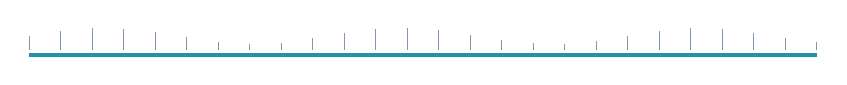
\begin{tikzpicture}
      \draw[insatcyan,very thick] (0,0)--(10,0);
      \foreach \x in {0,0.4,...,10} {
        \draw[insatblue!55] (\x,0.06) -- +(0,{0.18+0.10*sin(95*\x)});
      }
    \end{tikzpicture}
  \end{center}
\end{frame}

% =============================================================================
\begin{frame}{Problématique et objectifs}
  \begin{columns}[T,onlytextwidth]
    \column{0.51\textwidth}
      \begin{block}{Problème}
        Estimer directement la position 2D d'un utilisateur à partir de son
        empreinte radio :
        \[
          \mathbf H\in\mathbb C^{M\times K}
          \quad\longrightarrow\quad
          (\widehat{x},\widehat{y})
        \]
      \end{block}
      \vspace{0.15cm}
      \textbf{Pourquoi le CSI ?}
      \begin{itemize}
        \item sensible à la position et à la géométrie ;
        \item contient amplitude, phase, angles et retards ;
        \item disponible dans l'infrastructure radio.
      \end{itemize}

    \column{0.46\textwidth}
      \textbf{Objectifs}
      \begin{enumerate}
        \item Générer un dataset DeepMIMO réaliste.
        \item Construire un prétraitement sans fuite.
        \item Comparer CNN, ViT et hybride.
        \item Étudier multipath, bruit, antennes et sous-porteuses.
      \end{enumerate}
      \vspace{0.25cm}
      \keybox{Localisation = régression continue, pas classification}
  \end{columns}
\end{frame}

% =============================================================================
\begin{frame}{Que contient une matrice CSI ?}
  \begin{columns}[T,onlytextwidth]
    \column{0.54\textwidth}
      \begin{block}{Une entrée par utilisateur}
        \[
        \mathbf H=\left[H_{m,k}\right]
        \in\mathbb C^{64\times64}
        \]
        \[
        H_{m,k}=|H_{m,k}|e^{j\phi_{m,k}}
        \]
      \end{block}
      \begin{itemize}
        \item \textbf{64 antennes :} diversité spatiale et angulaire.
        \item \textbf{64 sous-porteuses :} diversité fréquentielle et retards.
        \item \textbf{Amplitude :} atténuation du canal.
        \item \textbf{Phase :} distance, déphasage et multipath.
      \end{itemize}

    \column{0.43\textwidth}
      \centering
      \includegraphics[width=0.88\linewidth]{../data/raw/o1_28_2d/csi_amplitude_db.png}
      \vspace{-0.1cm}
      \begin{center}
        \scriptsize Exemple d'amplitude CSI en dB
      \end{center}
      {\small\keybox{Le CSI agit comme une empreinte radio de la position}}
  \end{columns}
\end{frame}

% =============================================================================
\begin{frame}{Dataset DeepMIMO O1\_28}
  \begin{columns}[T,onlytextwidth]
    \column{0.53\textwidth}
      \centering
      \includegraphics[width=\linewidth]{../data/raw/o1_28_2d/user_positions.png}
    \column{0.40\textwidth}
      \begin{table}
        \scriptsize
        \setlength{\tabcolsep}{3.5pt}
        \begin{tabular}{ll}
          \toprule
          Paramètre & Valeur \\
          \midrule
          Fréquence & 28 GHz \\
          Bande OFDM & 50 MHz \\
          Utilisateurs & 10 000 \\
          Grille & $100\times100$ \\
          Zone & $\approx20\times20$ m \\
          Antennes BS & $8\times8$ \\
          Sous-porteuses & 64 \\
          Trajets max. & 10 \\
          CSI brut & complex64 \\
          \bottomrule
        \end{tabular}
      \end{table}
      \vspace{0.05cm}
      \begin{itemize}\scriptsize
        \item Ray tracing Wireless InSite.
        \item 10 000 CSI valides.
        \item Aucune position dupliquée.
        \item Aucun CSI nul ou non fini.
      \end{itemize}
  \end{columns}
\end{frame}

% =============================================================================
\begin{frame}{Prétraitement et découpage spatial}
  \begin{columns}[T,onlytextwidth]
    \column{0.49\textwidth}
      {\small\textbf{Transformation complexe $\rightarrow$ 3 canaux}}
      {\small\[
        \begin{aligned}
          X_1&=20\log_{10}|H|,\\
          X_2&=\cos(\angle H),\qquad X_3=\sin(\angle H)
        \end{aligned}
      \]}
      \vspace{-0.15cm}
      \begin{itemize}\small
        \item Le couple cos/sin évite la discontinuité $-\pi/\pi$.
        \item Standardisation ajustée sur le train uniquement.
        \item Coordonnées $(x,y)$ également standardisées.
      \end{itemize}
      \vspace{-0.05cm}
      \begin{table}
        \tiny
        \begin{tabular}{lrr}
          \toprule
          Région & Utilisateurs & Rôle \\
          \midrule
          Train & 6 800 & apprentissage \\
          Validation & 1 400 & sélection \\
          Test & 1 400 & résultat final \\
          Garde & 400 & anti-fuite \\
          \bottomrule
        \end{tabular}
      \end{table}

    \column{0.48\textwidth}
      \centering
      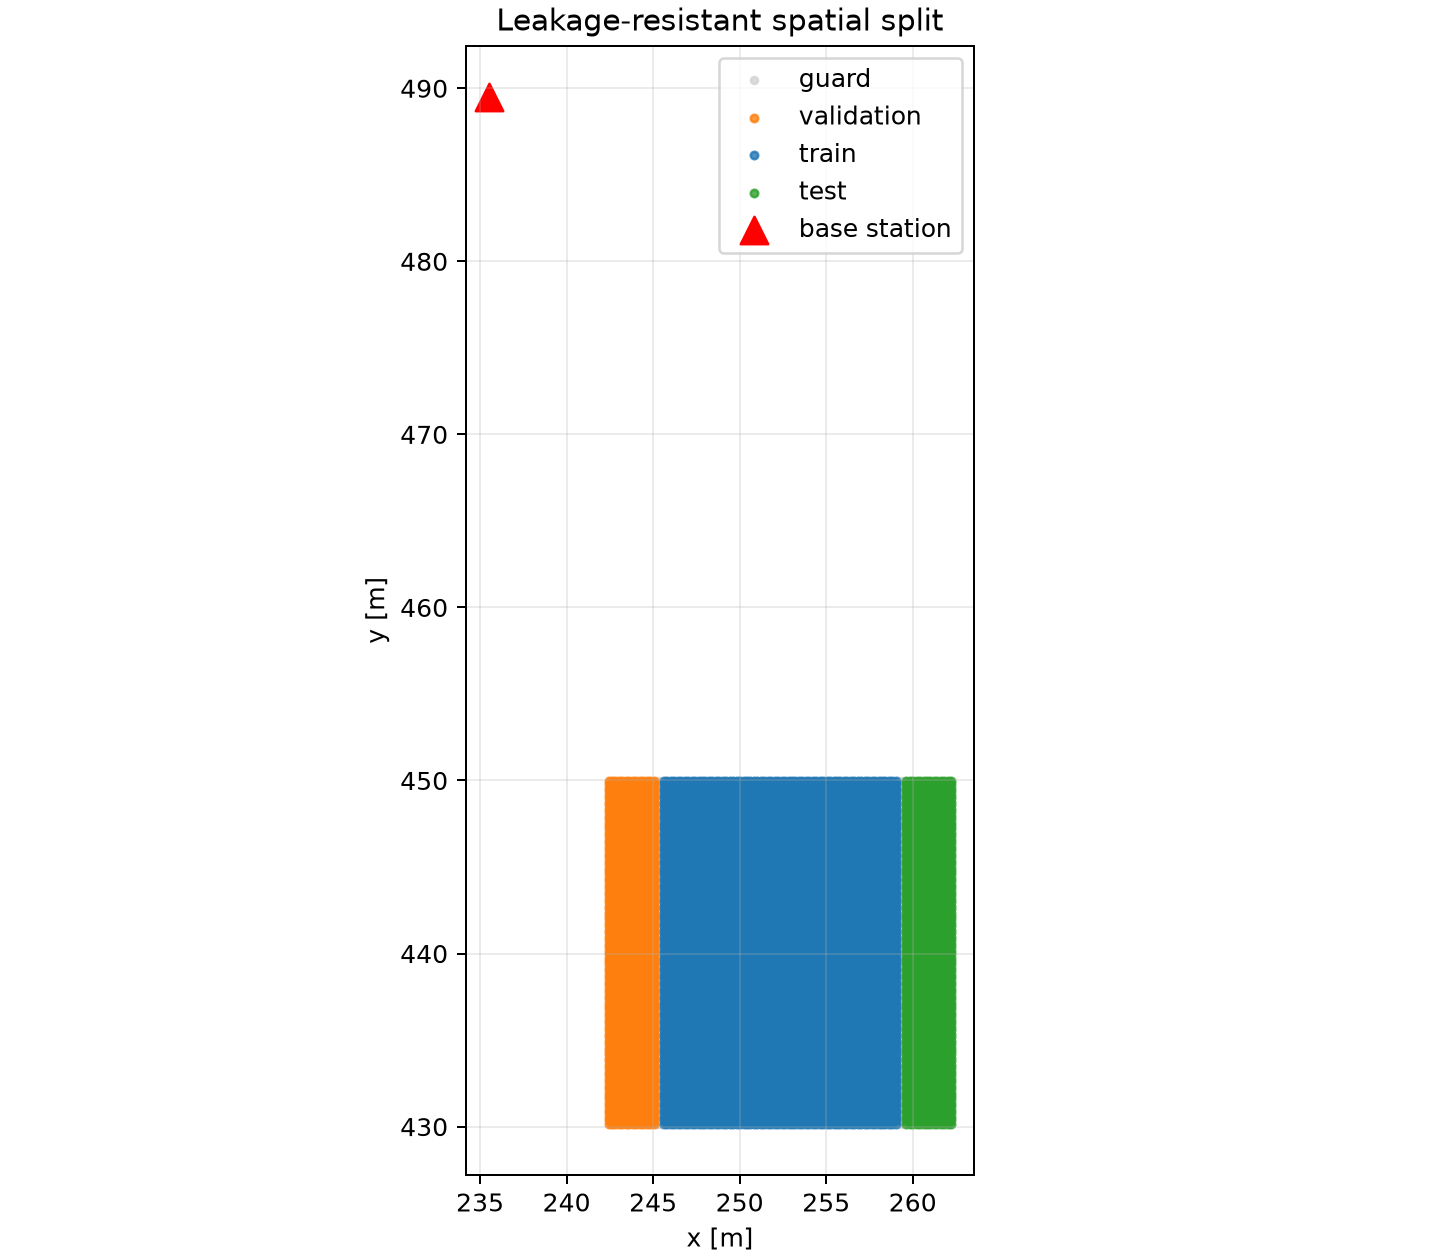
\includegraphics[width=0.82\linewidth]{../data/processed/o1_28_2d/spatial_split.png}
      \vspace{-0.1cm}
      {\small\keybox{Split spatial : pas de voisins quasi identiques entre train et test}}
  \end{columns}
\end{frame}

% =============================================================================
\begin{frame}{Architectures comparées}
  \begin{columns}[T,onlytextwidth]
    \column{0.29\textwidth}
      \begin{block}{CNN}
        \centering
        4 blocs convolutionnels\\
        16--32--64--96 canaux\\[0.2cm]
        Pooling global\\
        Régression $(x,y)$\\[0.25cm]
        \textbf{86 290 paramètres}
      \end{block}
      \centering\scriptsize Motifs locaux, rapide et compact

    \column{0.36\textwidth}
      \begin{block}{Vision Transformer}
        \centering
        Patches $8\times8$\\
        64 tokens + [CLS]\\
        Embedding 96\\
        4 blocs, 4 têtes\\[0.25cm]
        \textbf{329 090 paramètres}
      \end{block}
      \centering\scriptsize Relations globales antennes--fréquences

    \column{0.29\textwidth}
      \begin{block}{CNN--Transformer}
        \centering
        Stem convolutionnel\\
        24--48--96 canaux\\
        3 blocs Transformer\\[0.25cm]
        \textbf{289 754 paramètres}
      \end{block}
      \centering\scriptsize Extraction locale puis attention
  \end{columns}

  \vspace{0.45cm}
  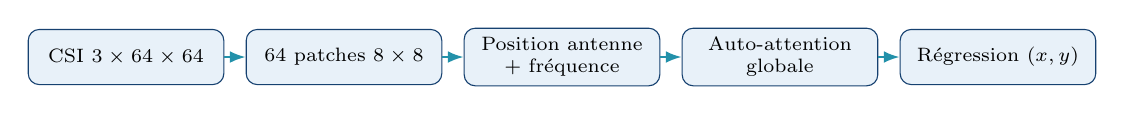
\begin{tikzpicture}[
    node distance=0.27cm,
    box/.style={draw=insatblue,rounded corners,fill=lightblue,
                minimum height=0.7cm,text width=2.25cm,align=center,font=\scriptsize},
    arrow/.style={-{Latex[length=2mm]},thick,insatcyan}
  ]
    \node[box] (in) {CSI $3\times64\times64$};
    \node[box,right=of in] (p) {64 patches $8\times8$};
    \node[box,right=of p] (e) {Position antenne + fréquence};
    \node[box,right=of e] (a) {Auto-attention globale};
    \node[box,right=of a] (o) {Régression $(x,y)$};
    \draw[arrow] (in)--(p); \draw[arrow] (p)--(e);
    \draw[arrow] (e)--(a); \draw[arrow] (a)--(o);
  \end{tikzpicture}
\end{frame}

% =============================================================================
\begin{frame}{Protocole expérimental}
  \begin{columns}[T,onlytextwidth]
    \column{0.49\textwidth}
      \textbf{Apprentissage}
      \begin{itemize}
        \item Régression des coordonnées normalisées.
        \item Perte MSE, optimiseur AdamW pour le ViT.
        \item Learning rate initial : $3\times10^{-4}$.
        \item Scheduler + early stopping.
        \item Graine fixée à 42.
        \item Meilleur ViT : époque 26.
      \end{itemize}

    \column{0.48\textwidth}
      \textbf{Évaluation en mètres}
      \[
        e_u=\sqrt{(\widehat{x}_u-x_u)^2+(\widehat{y}_u-y_u)^2}
      \]
      \begin{itemize}
        \item erreur moyenne ;
        \item médiane ;
        \item RMSE ;
        \item P90 et P95 ;
        \item courbe CDF.
      \end{itemize}
  \end{columns}
  \vspace{0.2cm}
  \keybox{Même test de 1 400 utilisateurs pour tous les modèles}
\end{frame}

% =============================================================================
\begin{frame}{Résultat principal : le ViT est le plus précis}
  \begin{columns}[T,onlytextwidth]
    \column{0.49\textwidth}
      \begin{table}
        \small
        \begin{tabular}{lrrr}
          \toprule
          Modèle & Moy. & Méd. & P90 \\
          \midrule
          Naïf & 10,270 & 10,083 & 12,487 \\
          CNN & 1,607 & 1,509 & 2,494 \\
          ViT & \best{0,970} & \best{0,883} & \best{1,794} \\
          Hybride & 1,818 & 1,707 & 2,935 \\
          \bottomrule
        \end{tabular}
      \end{table}
      \vspace{0.3cm}
      \begin{block}{Gain du ViT}
        \centering
        \Large \best{$-39,6\,\%$}\normalsize\\
        d'erreur moyenne par rapport au CNN
      \end{block}
      \scriptsize Toutes les erreurs sont exprimées en mètres.

    \column{0.48\textwidth}
      \includegraphics[width=\linewidth]{../outputs/comparison/all_models_test_cdf.png}
      \vspace{-0.1cm}
      \begin{itemize}
        \item CDF du ViT la plus à gauche.
        \item L'hybride perd probablement des détails lors du downsampling CNN.
      \end{itemize}
  \end{columns}
\end{frame}

% =============================================================================
\begin{frame}{Extension 1 : richesse du multipath}
  \begin{columns}[T,onlytextwidth]
    \column{0.40\textwidth}
      \begin{table}
        \small
        \begin{tabular}{rrr}
          \toprule
          Trajets & Moyenne & P90 \\
          \midrule
          1 & \best{0,715} & \best{1,409} \\
          3 & 0,749 & 1,446 \\
          5 & 1,612 & 2,502 \\
          10 & 0,970 & 1,794 \\
          \bottomrule
        \end{tabular}
      \end{table}
      \vspace{0.25cm}
      \begin{itemize}
        \item Même utilisateurs, split, ViT et graine.
        \item Un canal simple est plus facile à inverser.
        \item Résultat \textbf{non monotone}.
      \end{itemize}

    \column{0.57\textwidth}
      \includegraphics[width=\linewidth]{../outputs/multipath/comparison/multipath_metrics.png}
      \vspace{-0.15cm}
      \keybox{Conclusion prudente : le multipath modifie fortement la difficulté, sans loi générale démontrée}
  \end{columns}
\end{frame}

% =============================================================================
\begin{frame}{Extension 2 : robustesse au bruit complexe}
  \begin{columns}[T,onlytextwidth]
    \column{0.49\textwidth}
      \includegraphics[width=\linewidth]{../outputs/noise_robustness/mean_error_vs_snr.png}
      \vspace{-0.15cm}
      \scriptsize AWGN ajouté au CSI complexe avant le prétraitement.

    \column{0.48\textwidth}
      \begin{table}
        \scriptsize
        \begin{tabular}{lrrrr}
          \toprule
          Modèle & Propre & 20 dB & 10 dB & 0 dB \\
          \midrule
          CNN & 1,607 & 1,775 & 3,103 & 9,341 \\
          ViT & \best{0,970} & \best{0,997} & \best{1,358} & \best{3,767} \\
          Hybride & 1,818 & 1,862 & 2,327 & 10,760 \\
          \bottomrule
        \end{tabular}
      \end{table}
      \begin{itemize}
        \item Modèles gelés, entraînés sur CSI propre.
        \item 3 réalisations indépendantes par SNR.
        \item Dégradation faible à 20--30 dB.
        \item Le ViT reste meilleur jusqu'à 0 dB.
      \end{itemize}
      \keybox{0 dB : puissance du bruit = puissance du signal}
  \end{columns}
\end{frame}

% =============================================================================
\begin{frame}{Extension 3 : paramètres du système}
  \begin{columns}[T,onlytextwidth]
    \column{0.54\textwidth}
      \includegraphics[width=\linewidth]{../outputs/system_parameters/comparison/system_parameter_metrics.png}
    \column{0.43\textwidth}
      \begin{table}
        \scriptsize
        \begin{tabular}{lrr}
          \toprule
          Configuration & Moy. & P90 \\
          \midrule
          16 ant. / 64 sc. & 2,305 & 3,345 \\
          32 ant. / 64 sc. & 1,306 & 2,368 \\
          64 ant. / 64 sc. & \best{0,970} & \best{1,794} \\
          \midrule
          64 ant. / 16 sc. & 1,512 & 2,647 \\
          64 ant. / 32 sc. & 1,401 & 2,311 \\
          64 ant. / 64 sc. & \best{0,970} & \best{1,794} \\
          \bottomrule
        \end{tabular}
      \end{table}
      \begin{itemize}
        \item Antennes : $4\times4$, $4\times8$, $8\times8$.
        \item Sous-porteuses réparties sur les mêmes 50 MHz.
      \end{itemize}
      \keybox{Dans ce scénario, la diversité spatiale est la plus importante}
  \end{columns}
\end{frame}

% =============================================================================
\begin{frame}{Discussion : ce que les résultats permettent d'affirmer}
  \begin{columns}[T,onlytextwidth]
    \column{0.49\textwidth}
      \begin{block}{Enseignements}
        \begin{itemize}
          \item Le split spatial évite une évaluation optimiste.
          \item Le ViT exploite efficacement la structure globale du CSI.
          \item Son avantage persiste sous bruit.
          \item Antennes et sous-porteuses améliorent la précision.
        \end{itemize}
      \end{block}

    \column{0.48\textwidth}
      \begin{block}{Limites}
        \begin{itemize}
          \item Un seul scénario simulé.
          \item Une station et une hauteur fixe.
          \item Une seule graine d'entraînement.
          \item AWGN idéal, pas de défauts matériels.
          \item Pas encore de mesures CSI réelles.
        \end{itemize}
      \end{block}
  \end{columns}
  \vspace{0.3cm}
  \keybox{Résultat défendable : meilleur modèle sur notre protocole --- pas supériorité universelle du ViT}
\end{frame}

% =============================================================================
\begin{frame}{Conclusion et perspectives}
  \begin{columns}[T,onlytextwidth]
    \column{0.56\textwidth}
      \textbf{Bilan}
      \begin{itemize}
        \item Chaîne complète DeepMIMO $\rightarrow$ position 2D.
        \item 10 000 utilisateurs et split spatial strict.
        \item ViT : \best{0,970 m} de moyenne et \best{0,883 m} de médiane.
        \item ViT meilleur sur précision et robustesse au bruit.
        \item Études contrôlées du multipath et des paramètres radio.
      \end{itemize}

    \column{0.41\textwidth}
      \textbf{Perspectives}
      \begin{enumerate}
        \item Plusieurs graines et intervalles de confiance.
        \item Augmentation par bruit à l'entraînement.
        \item Généralisation inter-scénario.
        \item Mesures CSI réelles et mobilité.
        \item Compression pour le temps réel.
      \end{enumerate}
  \end{columns}
  \vspace{0.35cm}
  \begin{beamercolorbox}[rounded=true,sep=0.9em,center]{block title}
    \Large Le CSI peut devenir un capteur de position intégré au réseau 5G.
  \end{beamercolorbox}
\end{frame}

% =============================================================================
\begin{frame}[plain]
  \begin{center}
    \vspace{1.2cm}
    {\Huge\bfseries\color{insatblue} Merci pour votre attention}\par
    \vspace{0.7cm}
    {\LARGE Questions ?}\par
    \vspace{1.0cm}
    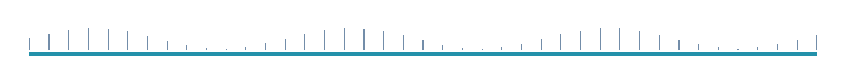
\begin{tikzpicture}
      \draw[insatcyan,very thick] (0,0)--(10,0);
      \foreach \x in {0,0.25,...,10} {
        \draw[insatblue!60] (\x,0.05) -- +(0,{0.15+0.13*sin(110*\x)});
      }
    \end{tikzpicture}
    \vfill
    {\large \Auteur\quad--\quad\Etablissement\quad--\quad2026--2027}
  \end{center}
\end{frame}

\end{document}
